\chapter{Sampling Methods}
\label{chap:sm}

\section{Inverse transform sampling}
\label{sec:sm:inverse_transform}

In the one-dimensional case, this amounts to converting a uniform random variable (which are easy to generate) into a variable sampled from a general distribution $f(\theta)$. One first finds its cumulative distribution function (CDF):
\begin{equation}
  F(\theta) = \int\limits_{-\infty}^\theta f(\theta^\prime) d\theta^\prime,
\end{equation}
computes the inverse of the CDF, and then applies this function to a uniform random variable  $x\sim U(0,1)$ to generate a variable $\theta = F^{-1}(x)$, which is distributed according to $f(\theta)$. 

In the general $D$-dimensional case, one calculates $D$ conditional distributions $\{f_i:i=1\ldots,D\}$: by marginalising over parameters with indices greater than $i$ and conditioning on parameters with indices less than $i$:
%
\begin{equation}
  f_i(\theta_i|\theta_{i-1},\ldots,\theta_1) 
  =
  \frac{%
    \int f_i(\params) d\theta_{i+1}\ldots d\theta_{N}
  }{%
    \int f_i(\params) d\theta_{i}\ldots d\theta_{N}
  },
\end{equation}
%
Integrating these yields $D$ conditional CDFs:
%
\begin{equation}
  x_i = F_i(\theta_i|\theta_{i-1},\ldots,\theta_1) = \int\limits_0^{\theta_i} f_i(\theta_i^\prime|\theta_{i-1},\ldots,\theta_1) d\theta_i^\prime.
\end{equation}
%
Inverting this gives $\theta_i = F^{-1}_i(x_i|\theta_{i-1},\ldots,\theta_1)$, which constitutes a set of relations sequentially transforming $D$ uniform random variables $\{x_i\}$ into $\{\theta_i\}$ distributed according to $f(\params)$.

In many cases, the prior $\prior(\params)$ is separable, and the above equations are easily calculated. For sections of the parameters which are not separable, the calculation can become more involved. We include a few demonstrations of this procedure in Section~\ref{sec:bay:prior_tranformations}. 



\section{Rejection Sampling}
\label{sec:sm:rejection}

\section{Importance Sampling}
\label{sec:sm:importance}

\section{Metropolis---Hastings}
\label{sec:sm:mh}
Metropolis---Hastings approaches are an extremely widely used methodology for generating a sequence of samples (or points) from some posterior $\posterior(x)$.

A sequence of $T$ points is termed a {\em chain\/} $\chain_T$:
\begin{equation}
  \chain_T = \{ x^{(t)}: t=1\cdots T \}
\end{equation}
A new point $x^{(t+1)}$ is generated from a proposal density $\proposal$ which depends on the current state $x^{(t)}$. Typically $\proposal(x|x^{(t)})$ might be a Gaussian distribution centered on the current value of $x^{(t)}$:
\begin{equation}
  \log \proposal(x|x^{(t)}) = \text{const} -\frac{{\left[ x-x^{(t)} \right]}^2}{2\varepsilon^2},
\end{equation}
but in general the proposal density can be any fixed density from which we may draw samples easily.

A new state $x$ is proposed from the proposal density $\proposal(x|x^{(t)})$, and it is accepted with probability:
\begin{equation}
  p_\mathrm{accept}(x|x^{(t)}) = \frac{\posterior(x)}{\posterior(x^{(t)})}\frac{\proposal(x^{(t)}|x)}{\proposal(x|x^{(t)})}.
\end{equation}
If the step is accepted, then $x^{(t+1)}=x$, otherwise $x^{(t+1)} = x^{(t)}$. This procedure can be seen schematically in Figure~\ref{fig:sm:MH}.
\begin{figure}
  \centering
  \begin{tikzpicture}
   %\draw [rotate=30, x radius=4, y radius=1, delta angle=360] (0,0)
    %arc [start angle=0];

  \draw[rotate=30, dotted] (0,0) ellipse (4 and 1);
  \draw[rotate=30, dotted] (0,0) ellipse (2 and 0.5);
  \draw[rotate=30, dotted] (0,0) ellipse (1 and 0.25);
  \draw[rotate=30, dotted] (0,0) ellipse (0.5 and 0.125);
  \draw[] (0,1.4)  node {\(\posterior\)};
  \draw[] (-2,0)  node[above left]  {\(\proposal\)};

  \coordinate (circ) at (-2,-1);
  \draw[dashed] (circ) circle (1);

  \draw[fill=black] (circ) circle (0.05);

  \draw[-latex] (circ) -- +(135:1) ;
  \draw[-latex] (circ) -- +(0:1);
  \draw[-latex] (circ) -- +(-90:1) node [midway,left] {\(\varepsilon\)};


  \draw[] (circ) node [above right] {\(x^{(t)}\)};

  \draw[latex-latex] ($(30:4) + (-60:2)$)  --  +(30:-8) node[midway,below right] {\(\sigma_{\max{}}\)};

  \draw[latex-latex] ($(120:1) + (30:5)$)  --  +(120:-2) node[midway,above right] {\(\sigma_{\min{}}\)};
\end{tikzpicture}


  \caption{Metropolis---Hastings. Here we have some degenerate two-dimensional posterior $\posterior$, and a circular proposal distribution $\proposal$.\label{fig:sm:MH}}.
\end{figure}


This has the distinct advantage that it does not require one to take into account the overall normalisation of the posterior, circumnavigating any issues associated with computing the evidence $\evidence$, since:
\begin{equation}
  \frac{\posterior(x)}{\posterior(x^{(t)})} \equiv
  \frac{\lik(x)\prior(x)}{\lik(x^{(t)})\prior(x^{(t)})} 
\end{equation}
It is important to note that the chain $C_T$ will comprise $T$ samples which are {\em correlated}. If the proposal distribution amounts to a random walk with step size $\varepsilon<\sigma_{\min{}}$, and the longest lengthscale in the probably region is $\sigma_{\max{}}$  then one will expect: $\tau \sim {(L/\varepsilon)}^2$. If $\varepsilon>\sigma_{\min{}}$, then one starts to expect a very low acceptance rate, so typically for a isotropic random walk, the timescale on which one expects to generate independent samples is:
\begin{equation}
  \tau \sim \left( \frac{\sigma_{\max{}}}{\sigma_{\min{}}} \right).
\end{equation}
In theory, given that the above relation has no dimensionality attached to it, Metropolis Hastings can be extremely successful in high dimensions. However, there are several issues.

First, one does not initially a-priori have a good starting point. There is therefore a period of ``burn-in'' attached to MH methods. Knowing when this period is truely over, and one is starting to generate random samples can be challenging in the general case.

In many cases, $\tau\gg1$ resulting in unacceptable run-times. This can be ameliorated by choosing a proposal distribution $\proposal$ that better agrees with the posterior $\posterior$. However, this amounts to adding in many effective tuning parameters. Many algorithms work by having a ``learning'' phase, whereby the algorithm deduces for itself a good correlated Gaussian proposal distribution, but given the fact that this is not strictly Markovian care must be taken.



\section{Gibbs Sampling}


\section{Slice sampling}
\label{sec:sm:slice}
Radford Neal initially proposed slice sampling as an effective methodology for generating samples numerically from a given posterior $\posterior(\params)$. One first chooses a `slice' (or probability level) $\posterior_0$ uniformly within $[0,\posterior_\smax]$. One then samples uniformly within the $\params$-region defined by $\posterior(\params)>\posterior_0$. The similarity with the iso-likelihood contour sampling required by nested sampling should be clear. In the one-dimensional case, he suggests the sampling procedure detailed in Figure~\ref{fig:bay:1d_slice}.

\begin{figure}
  \centerline{%
    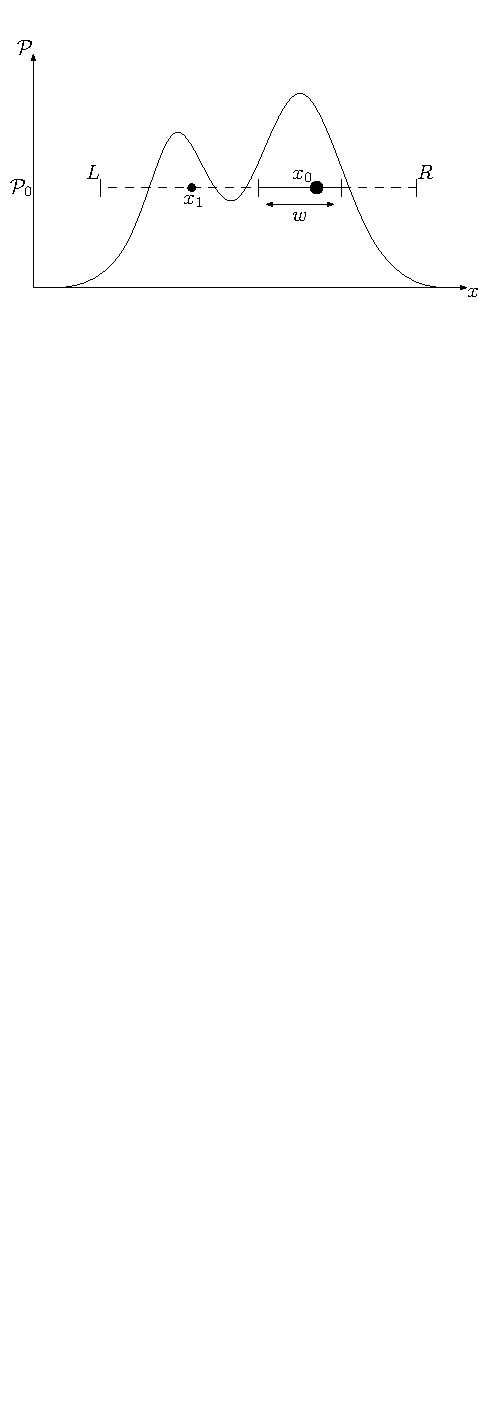
\includegraphics[width=\textwidth]{slice}
  }

  \caption{Slice sampling in one dimension. 
    Given a probability level (or slice) $\posterior_0$, slice sampling samples within the horizontal region defined by $\posterior>\posterior_0$. 
    From an initial point $x_0$ within the slice ($\posterior(x_0)>\posterior_0$), a new point $x_1$ is generated within the slice with a distribution $P(x_1|x_0)$.
    External bounds are first set on the slice $\hat{L}<x_0<\hat{R}$ by uniformly expanding a random initial bound of width $w$ until they lie outside the slice (Neal terms this the {\em stepping out\/} procedure). 
    $x_1$ is then sampled uniformly within these bounds.  
    If $x_1$ is not in the slice, then $\hat{L}$ or $\hat{R}$ is replaced with $x_1$, ensuring that $x_0$ is still within the slice.
    This procedure is guaranteed to generate a new point $x_1$, and satisfies detailed balance $P(x_0|x_1) = P(x_1|x_0)$. Thus, if $x_0$ is drawn from a uniform distribution within the slice, so is $x_1$.\label{fig:bay:1d_slice}
  }
\end{figure}



In higher dimensions,~\cite{NealSlice} suggests a variety of MCMC-like methods. The simplest of these is implemented by sampling each of the parameter directions in turn. Since each one-dimensional slice requires $\bigO{\text{a few}}$ likelihood calculations, the number of likelihood calculations required scales linearly with dimensionality, providing the region is efficiently navigated. Multi-dimensional slice sampling has many of the benefits of a traditional MH approach, and uses a proposal distribution which is much more efficient at sampling a hard likelihood constraint.
